% !TeX program=xelatex
\documentclass{ctexart}
\usepackage{comment}

\setCJKmainfont[BoldFont = Adobe Heiti Std, ItalicFont = Adobe Kaiti Std R]{宋体}
% 无衬线字体同上
\setCJKsansfont[BoldFont = Adobe Heiti Std, ItalicFont = Adobe Kaiti Std R]{宋体}

% For figures
\usepackage{graphicx}
\usepackage{subfigure} 

% For citations
\usepackage{natbib}

% For algorithms
\usepackage{algorithm}
\usepackage{algorithmic}

\usepackage{hyperref}

\newcommand{\theHalgorithm}{\arabic{algorithm}}

\usepackage[accepted]{icml2017}

\usepackage{amsmath,amssymb,amsthm}
\DeclareMathOperator*{\argmax}{arg\,max}
\DeclareMathOperator*{\argmin}{arg\,min}

\def\bR{\mathbb{R}}

\def\cB{\mathcal{B}}
\def\cD{\mathcal{D}}
\def\cN{\mathcal{N}}
\def\cX{\mathcal{X}}
\def\cZ{\mathcal{Z}}

\def\vl{\mathbf{l}}
\def\vx{\mathbf{x}}
\def\vy{\mathbf{y}}
\def\vz{\mathbf{z}}
\def\vp{\mathbf{p}}
\def\vq{\mathbf{q}}

\def\defeq{\overset{\mathrm{def}}{=}}

\icmltitlerunning{Connectionist Temporal Classification}

\begin{document} 

\twocolumn[
\icmltitle{联结主义时序分类:\\用循环递归网络分类未切分的序列数据}

\begin{icmlauthorlist}
\icmlauthor{Alex Graves}{idsia}
\icmlauthor{Santiago Fern\'andez}{idsia}
\icmlauthor{Faustino Gomez}{idsia}
\icmlauthor{J\"urgen Schmidhuber}{idsia,tum}
\end{icmlauthorlist}

\icmlaffiliation{idsia}{Istituto Dalle Molle di Studi sull’Intelligenza Artificiale (IDSIA), Galleria 2, 6928 Manno-Lugano, Switzerland}
\icmlaffiliation{tum}{Technische Universit\"at München (TUM), Boltzmannstr. 3, 85748 Garching, Munich, Germany}

\icmltranslator{张远航}{me@caszhang.cn}
\icmlkeywords{CTC, sequence labelling}

\vskip 0.3in
]

\printAffiliationsAndNotice{}

\begin{abstract} 
现实生活中的许多序列学习任务涉及从含噪声、未切分的输入数据中产生序列的分类预测.例如,在语音识别当中,声学信号会被切分为字或更小的单元.作为强大的序列学习器,循环神经网络看起来似乎很适合这种任务,但它们需要已经切分好的训练数据,还需要后处理来将输出转变为标签序列,因此它们的应用场景目前为止还是比较有限的.本文提出一种新方法训练循环神经网络,直接对未标注的序列做分类,从而解决了以上两个问题.在~TIMIT~语音语料库上的实验证明它相较基准~HMM~模型和~HMM-RNN~混合模型都有优势.
\end{abstract} 

\section{引言}
\label{sec:intro}
在现实生活里的序列学习中,为未切分的(unsegmented)序列数据做分类是一个很常见的问题.在感知类(perceptual)任务当中,它尤其常见(例如手写体识别、语音识别和手势识别).我们需要将含噪声的实值输入流用字或词之类的离散标签串进行标注(annotate).

当下,图模型是序列标注任务的主流框架,例如隐马尔可夫模型(hidden Markov model, HMM; \citealp{rabiner1989tutorial})、条件随机场(conditional random field, CRF; \citealp{lafferty2001conditional})以及它们的变种.尽管这些方法成功解决了许多问题,它们还存在几个缺陷:(1)它们通常要求大量的与领域相关的知识,例如为~HMM~设计状态模型,或者为~CRF~选择输入特征;(2)它们要求显式(有时候还不合理)的依赖性条件(dependency assumptions),从而使得推断问题易解(tractable),例如,HMM~当中假设观察是相互独立的;(3)对于标准的~HMM~来说,训练是生成式的,但序列分类(sequence labelling)
\footnote{本文参照《序列标注中的神经网络方法研究》[吴惠甲, 宗成庆 2017]一文,将``sequence labelling"译为“序列分类”,而中文的“序列标注”一词则对应于``sequence tagging".宏观上二者均为序列中的每个词产生一个标签,其区别或许可以理解为,分类根据当前特征确定当前类别,无需考虑上下文的分类结果;而标注所采集的特征里面有上下文分类结果.CTC~作为一种端到端的建模方式显然属于前者.——译者}
本身是一个判别式任务.

循环神经网络则不同,它不要求对数据的先验知识,只需要知道输入和输出表示.其内部的状态可以判别式地训练,从而为时间序列建模提供了一种强大通用的机制.此外,它们对于时间和空间上的噪声通常是比较鲁棒的.

然而目前为止,人们还未能将~RNN~直接应用于序列分类.问题在于,一般的神经网络目标函数是为训练序列当中的每个点单独定义的;换句话说,RNN~只能用来在一系列独立的标签分类上进行训练.这意味着输入数据必须是预先切分好的,而网络输出也要经过后处理才能给出最后的标签序列.

当下,在序列标注中~RNN~最有效的用法是和~HMM~合在一起实现所谓的混合式方法(hybrid approach; \citealp{bourlard1994connectionist}; \citealp{bengio1999markovian}).混合式系统用~HMM~对数据的长时间序列结构进行建模,定位后神经网络负责给出各分类.HMM~这一部分可以自动将序列在训练过程中进行切分,并将网络的分类转化为标签序列.然而混合系统不但具有上面提到的~HMM~的缺点,也没有完全发挥出~RNN~在序列建模方面的潜力.

本文提出一种新的方法对数据用~RNN~进行序列分类,既不需要对训练数据进行预切分,也不需要对输出进行后处理,用一个网络框架就可以对整个序列的各个方面进行建模.基本的想法是把网络输出视作给定输入序列,在所有可能的标签序列上的一个条件概率分布.有了这个概率分布,就可以导出一个目标函数,直接最大化正确标签的概率.由于目标函数是可导的,网络可以用标准的时间反向传播算法(backpropagation through time; \citealp{werbos1990bptt})进行训练.

接下来,我们将标注未切分的数据序列这一任务称为\textbf{时序分类}(temporal classification; \citealp{kadous2002temporal}),并将我们对RNN的这一使用方法称为\textbf{联结主义时序分类}(connectionist temporal classification, CTC).与之对比的,我们将在每个时间步(time-step)---或称帧(frame)---进行独立标注的任务称为\textbf{逐帧分类}(framewise classification).

下一节中给出了时序分类的数学形式化,并定义了本文中用到的误差度量.第~\ref{sec:ctc}~节描述了使得~RNN~能够被用作时序分类器的输出表示.第~\ref{sec:training}~节描述了如何训练~CTC~网络.第~\ref{sec:experiments}~节将~CTC~与混合式系统和~HMM~系统在~TIMIT~语音语料库上进行比较.第~\ref{sec:discussion}~节讨论了~CTC~和其他时序分类器的一些关键区别,指明了未来的工作方向.第~\ref{sec:conclusion}~节对本文做总结.
\section{时序分类}
令$S$为从一固定分布$\cD_{\cX\times\cZ}$中取出的训练样本集.输入空间是所有$m$维实值向量的集合$\cX = (\bR^m)^*$.目标空间是标签的(有限)字母表$L$上所有可能序列的集合$\cZ = L^*$.一般我们称$L^*$中的元素为\textbf{标签序列}(label sequence)或\textbf{标注}(labelling).$S$中每个样本是一个序列对$(\vx, \vz)$.目标序列$\vz = (z_1,z_2,\dots, z_U)$的长度不超过输入序列$\vx = (x_1,x_2,\dots,x_T)$,即$U\le T$.输入和输出序列通常不等长,因此没有对齐它们的\textbf{先验}方法.

目标是用$S$训练一个时序分类器$h:\cX\mapsto\cZ$,最小化某个与任务相关的错误度量,并用它对之前未见过的输入序列进行分类.
\subsection{标签错误率}
\label{sec:ler}
本文中,我们感兴趣的是下述错误度量:给定一个与$S$不相交的测试集$S'\subset\cD_{\cX\times\cZ}$,定义时序分类器$h$的\textbf{标签错误率}(label error rate, LER)为分类和$S'$中目标的归一化编辑距离(normalised edit distance),即
\begin{equation}
	\textit{LER}(h, S') = \frac 1Z \sum_{(\vx, \vz)} \textit{ED}(h(\vx))
\end{equation}
其中$Z$是$S'$中标签的总数,$\textit{ED}(\vp,\vq)$是序列$\vp$和$\vq$之间的编辑距离,即将$\vp$变为$\vq$所需要的最少的增删和替换次数.

对于以最小化转写(transcription)错误率为目标的任务(如语音识别和手写体识别),这是一个很自然的度量.
\section{联结主义时序分类}
\label{sec:ctc}
本节描述为让循环神经网络进行~CTC~所采用的输出表示.关键步骤是将网络输出转化为一个关于标签序列的条件概率分布.之后,对输入序列选取最概然标注,就可以把网络当做分类器使用.
\subsection{从网络输出到标注}
CTC~网络中有一个~softmax~输出层\citep{bridle1990probabilistic},该层所包含的单元数是$L$中标签的个数加一.前$|L|$个单元单元的激活值应理解为在某一给定时刻观测到相应标签的可能性.额外单元的激活值(activation)是观测到一个“空符号”(`blank'),即没有标签的情况的概率.这些输出值定义了所有把标签序列和输入序列进行对齐的可能方式对应的概率.要求出任何一个可能标签序列的概率,我们就可以把它们的不同的对齐方式求和,得出相应的概率.

更正式的表述如下:对长为$T$的输入序列$\vx$,我们把有$m$个输入、$n$个输出和权重向量$w$的循环神经网络定义为一个连续映射$\cN_w:(\bR^m)^T\mapsto (\bR^n)^T$.设$\vy = \cN_w(\vx)$为网络输出的序列,并记输出单元$k$在时刻$t$的激活值为$y_k^t$,则$y_k^t$应理解为在时刻$t$观测到标签$k$的概率,它确定了$L'^T$上的一个概率分布,这里$L'^T$是字母表$L'=L\cup\{\textit{blank}\}$上长为$T$的序列所构成的集合:
\begin{equation}
	\label{eq:2}
	p(\pi|\vx) = \prod_{t=1}^{T} y_{\pi_t}^t, \forall\pi\in L'^T.
\end{equation}
从现在起,我们称$L'^T$中的元素为\textbf{路径}(path),并将其记为$\pi$.

\eqref{eq:2}~式中隐含的假设是,给定网络的内部状态,网络在不同时刻的输出间是相互条件独立的.这点是通过要求输出层到自身和网络均没有前馈连接(feedback connection)来保证的.

下一步是定义一个多对一映射$\cB: L'^T\mapsto L^{\le T}$,其中$L^{\le T}$是所有可能标注构成的集合(例如,所有原始标签字母表$L$上不长于$T$的字符串).为此,我们从路径中除去所有的空字符和重复的标签(例如,$\cB(a-ab-)=\cB(-aa--abb)=aab$).直观上,这相当于只在网络不再预测无标签或预测的标签发生变化时输出一个新标签(见图~\ref{fig:1}~中~CTC~的输出).最后,我们借助$\cB$,定义某给定标签$\vl\in L^{\le T}$的条件概率为其所有对应路径的概率之和:
\begin{equation}
	\label{eq:3}
	p(\vl|\vx) = \sum_{\pi\in\cB^{-1}(\vl)}p(\pi|\vx).
\end{equation}
\begin{figure*}
	\label{fig:1}
	\centering
	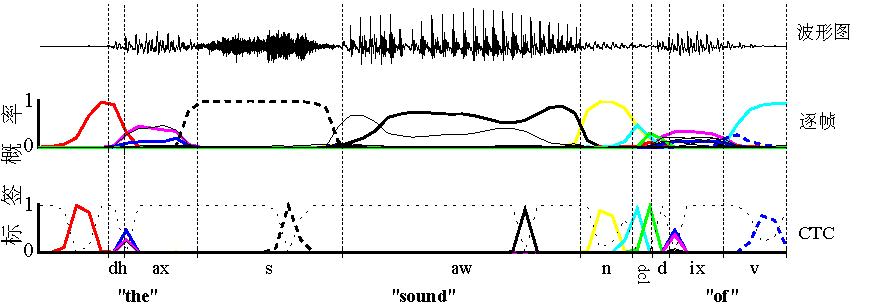
\includegraphics[width=\textwidth]{fig/1}
	\caption{\textbf{对一段语音信号进行逐帧分类和~CTC~网络分类}.带颜色的线代表对应于某时刻观察到某音素概率的输出激活值. CTC~网络只预测音素序列(通常是以一系列尖峰的形式,中间以空字符即空预测分隔),而逐帧分类的网络尝试将它们与人工切分的结果进行对齐(竖线).即使音素预测正确(如`dh'),逐帧网络也会收到切分边界未对齐的误差信号.如果某个音素总出现在另一个音素旁(如闭合[closure] `dcl'和塞音[stop] `d'),那么~CTC~会把它们以一个双峰的形式一同预测出来.标注的选择可以(依照双峰)从~CTC~的输出直接读出,而逐帧网络的结果必须进行后处理才能使用.}
\end{figure*}
\subsection{构造分类器}
\label{sec:classifier}
有了上面的表述,分类器的输出就应该是输入序列的最概然标注:
\[h(\vx) = \argmax_{\vl\in L^{\le T}} p(\vl|\vx).\]
我们采用~HMM~的术语,称寻找这一标注的任务为\textbf{解码}(decoding).可惜就我们所知,没有适用于这一系统的通用、具有易解性的解码算法.不过下面两种近似方法在实践中表现不错.

第一种方法(最优路径解码,best path decoding)基于最概然路径对应最概然标签的假设:
\begin{equation}
	\begin{split}
		h(\vx) & \approx \cB(\pi^*)\\
		\text{其中}~\pi^* & = \argmax_{\pi\in N^t}p(\pi|\vx).
	\end{split}
\end{equation}
最优路径解码的计算是平凡的,因为$\pi^*$不过是把每个时间步的最活跃输出拼接起来.然而这一方法并不一定能找到最概然标注.

第二种方法(前缀搜索解码,prefix search decoding)依赖于这一事实:对~\ref{sec:forward-backward}~节的前向-后向算法加以修改,就能逐步扩展,高效计算出标注各前缀的概率(图~\ref{fig:2}).
\begin{figure}
	\label{fig:2}
	\centering
	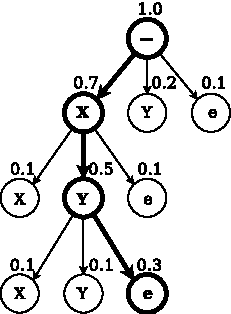
\includegraphics[width=0.5\columnwidth]{fig/2}
	\caption{\textbf{在标签的字母表$\mathrm{X}, \mathrm{Y}$上进行前缀搜索解码}.每个结点要么扩展父结点的前缀,要么终结(`$\mathrm{e}$').上图中各扩展结点上的数值代表所有以该前缀开始的标注的全概率.终结结点上方的数值是在其父结点结束的标注对应的概率.每轮迭代时,扩展剩下的最概然前缀.当找到某个概率比余下的前缀都大的标注(这里是`$\mathrm{XY}$')时终止搜索.}
\end{figure}

如果时间足够,前缀搜索解码总能找到最概然标注.然而算法所需扩展前缀的最大数目随输入序列的长度指数级增长.如果输出以较尖峰的方式分布在模(mode)附近,算法还是能在可接受的时间内结束的.不过对于本文中的实验,还需进一步增加启发式规则(heuristics)才能应用这一算法.
% TODO:启发式-规则?函数?方法?

训练好的~CTC~网络的输出通常倾向于形成一系列尖峰,中间以预测概率极高的空符号分隔(图~1).观察到这一点,我们将输出序列分为若干很可能以空符号开始或结尾的小段.为此,我们选出观测到空符号的概率大于某固定阈值的区间端点.接下来我们对每段计算最概然标注,并将它们拼接起来得到最终的分类结果.

实践中,带启发式规则的前缀搜索效果不错,而且通常比最优路径解码要好.不过某些情况下它也会失效,比如某段两个端点侧预测的标签相同,但置信都比较弱.
\section{网络训练}
\label{sec:training}
目前我们已经描述了可以使得~RNN~用于~CTC~的输出表示,现在我们为训练~CTC~网络导出一个目标函数,使得它可以用梯度下降法训练.这一目标函数是从最大似然原理导出的.也就是说要最小化这些函数,就要最大化目标标签的对数自然.注意到这和一般的神经网络目标函数\citep{bishop1995neural}背后的原理是一样的.给定一个目标函数以及它相对于网络输出的导数之后,权重的梯度就可以用标准的时间反向传播算法计算.接着网络就可以用任意当前在神经网络中使用的基于梯度的优化算法(\citealp{lecun1998efficient}; \citealp{schraudolph2002fast})进行训练.

我们首先来看一个求极大似然所必需的算法.
\subsection{CTC~的前向-后向算法}
\label{sec:forward-backward}
我们需要一种高效算法来计算各个标注的条件概率$p(\vl|\vx)$.一眼望去,\eqref{eq:3}~式表明这个是棘手的问题:求和是要对一个给定的标注所有的可能路径进行的,而一般来说,这样的路径有很多条.

幸运的是,这个问题可以用动态规划(dynammic programming)算法来解决,类似于~HMM~模型中的前向-后向算法(forward-backward algorithm).核心思想是对于一个标注,在所有路径上求和可以分解为对这一标注各前缀所对应路径的迭代求和.迭代的过程可以用递归的\textbf{前向}和\textbf{后向}变量高效计算.

对于某个长度为$r$的序列$\vq$,将其前$p$个和最后$p$个符号分别记为$\vq_{1:p}$和$\vq_{r-p:r}$.接着,定义标注$\vl$的前向变量$\alpha_t(s)$为时刻$t$的全概率,即
\begin{equation}
	\label{eq:5}
	\alpha_t(s)
	\defeq
	\sum_{
		\substack{
			\pi\in N^T:\\
			\cB(\pi_{1:t}) = \vl_{1:s}
		}
	}
	\prod_{t'=1}^t y_{\pi_{t'}}^{t'}.
\end{equation}
我们很快就会看到,$\alpha_t(s)$可由$\alpha_{t-1}(s)$和$\alpha_{t-1}(s-1)$递归求出.

为了允许在输出路径中包含空字符,我们考虑经过修改的标签序列$\vl'$,它由在头尾和每两个标签之间增加一个空字符得到.因此,$\vl'$的长为$2|\vl|+1$.计算$\vl'$各前缀的概率时,我们允许空标签和其他标签之间的任意转移,也允许任意\textbf{不同的}非空标签之间的转移.任意前缀只允许以空字符($b$)或$\vl$的第一个字符($\vl_1$)开始.

这样就有了下面的初始化规则
\begin{equation*}
	\begin{split}
		\alpha_1(1) & = y_b^1\\
		\alpha_1(2) & = y_{\vl_1}^1\\
		\alpha_1(s) & = 0, \forall s > 2
	\end{split}
\end{equation*}
和递归关系
\begin{equation}
	\label{eq:6}
	\alpha_t(s) = 
	\begin{cases}
		\bar{\alpha}_t(s) y_{\vl_s'}^t
		\hfill \text{若}~\vl_s' = b~\text{或}~\vl_{s-2}'=\vl_s'\\
		\big(\bar{\alpha}_t(s) + \alpha_{t-1}(s-2)\big) y_{\vl_s'}^t  
		\hfill \text{其他情况}
	\end{cases}
\end{equation}
其中
\begin{equation}
	\label{eq:7}
	\bar{\alpha}_t(s)
	\defeq
	\alpha_{t-1}(s) + \alpha_{t-1}(s-1).
\end{equation}
注意到$\alpha_t(s) = 0~\forall s<|\vl'|-2(T-t)-1$,因为这些变量对应于剩余时间步不够完成序列的那些状态(图~\ref{fig:3}~右上角无连接的圆圈).此外,$\alpha_t(s) = 0 \forall s<1$.
\begin{figure}
	\label{fig:3}
	\centering
	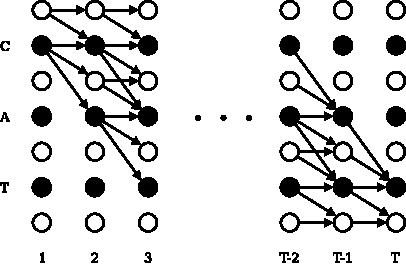
\includegraphics[width=0.9\columnwidth]{fig/3}
	\caption{\textbf{在标注`CAT'(猫)上应用前向-后向算法的图示}. 黑色的圆圈代表标签,白色的圆圈代表空符号.箭头代表允许的转移.前向变量沿箭头方向更新,后向变量逆着箭头方向更新.}
\end{figure}

这样,$\vl$的概率就是$\vl'$在时刻$T$结尾有空字符和无空字符的全概率.
\begin{equation}
	\label{eq:8}
	p(\vl|\vx) = \alpha_T(|\vl'|) + \alpha_T(|\vl'|-1).
\end{equation}
类似地定义后向变量$\beta_t(s)$为$\vl_{s:|\vl|}$在$t$时刻的全概率.
\begin{equation}
	\label{eq:9}
	\beta_t(s)
	\defeq
	\sum_{
		\substack{
			\pi\in N^T:\\
			\cB(\pi_{t:T}) = \vl_{s:|\vl|}
		}
	}
	\prod_{t'=t}^T y_{\pi_{t'}}^{t'}.
\end{equation}

\begin{equation*}
	\begin{split}
		\beta_T(|\vl'|) & = y_b^T\\
		\beta_T(|\vl'|-1) & = y_{\vl_{|\vl|}}^T\\
		\beta_T(s) & = 0, \forall s < |\vl'|-1
	\end{split}
\end{equation*}

\begin{equation}
	\label{eq:10}
	\beta_t(s) = 
	\begin{cases}
		\bar{\beta}_t(s) y_{\vl_s'}^t
		\hfill \text{若}~\vl_s' = b~\text{或}~\vl_{s+2}'=\vl_s'\\
		\big(\bar{\beta}_t(s) + \beta_{t+1}(s+2)\big) y_{\vl_s'}^t  
		\hfill \text{其他情况}
	\end{cases}
\end{equation}
其中
\begin{equation}
	\label{eq:11}
	\bar{\beta}_t(s)
	\defeq
	\beta_{t+1}(s) + \beta_{t+1}(s+1).
\end{equation}
注意,$\beta_t(s) = 0~\forall s > 2t$(图~3~左下角无连接的圆圈)、$\forall s > |\vl'|$.
实践中,上述递归很快就会导致计算机发生下溢(underflow).要避免这种情况,一种方式是缩放(rescale)前向和后向变量\citep{rabiner1989tutorial}.如果我们定义
\[C_t \defeq \sum_s\alpha_t(s), 
\quad \hat{\alpha}_t(s)\defeq\frac{\alpha_t(s)}{C_t}\]
并在~\eqref{eq:6}~和~\eqref{eq:7}~的右侧以$\hat{\alpha}$代$\alpha$,前向变量就可保持在可计算范围内.类似地我们对后向变量定义
\[D_t \defeq \sum_s\beta_t(s), 
\quad \hat{\beta}_t(s)\defeq\frac{\beta_t(s)}{C_t}\]
并在~\eqref{eq:10}~和~\eqref{eq:11}~的右侧以$\hat{\beta}$代$\beta$.
为了计算最大似然误差,我们需要求目标标注概率的自然对数.利用缩放后的变量表达,形式非常简单:
\[\ln{(p(\vl|\vx))} = \sum_{t=1}^T \ln{(C_t)}\]
\subsection{最大似然训练}
最大似然训练的目标是将训练集中所有正确分类的对数概率同时最大化.本文中,这意味着要最小化下面的目标函数:
\begin{equation}
	\label{eq:12}
	O^{\textit{ML}}(S,\cN_w) = -\sum_{(\vx,\vz)\in S}\ln{(p(\vz|\vx))}
\end{equation}
为了使用梯度下降训练网络,我们需要对~\eqref{eq:12}~关于网络的输出求导.由于训练样本是互相独立的,我们可以分别考虑:
\begin{equation}
	\label{eq:13}
	\frac{\partial O^{\textit{ML}}(\{(\vx,\vz)\},\cN_w)}{\partial y_k^t} = -\frac{\partial \ln{(p(\vz|\vx))}}{\partial y_k^t}
\end{equation}
下面我们说明如何利用~\ref{sec:forward-backward}~中的算法计算~\eqref{eq:13}.

核心是,对标注$\vl$,给定符号$s$和时刻$t$,则此时的前向和后向变量之积就是所有对应$\vl$,且在$t$时刻经过$s$的路径的概率之和.更准确地说,由~\eqref{eq:5}~和~\eqref{eq:9}~得:
\[
	\alpha_t(s)\beta_t(s)
	\defeq
	\sum_{
		\substack{
			\pi\in\cB^{-1}(\vl):\\
			\pi_t = \vl_s'
		}
	}
	y_{\vl_s'}^t
	\prod_{t=1}^T y_{\pi_t}^t.
\]
整理,将~\eqref{eq:2}~代入,得
\[\frac{\alpha_t(s)\beta_t(s)}{y_{\vl_s'}^t} = 
	\sum_{
		\substack{
			\pi\in\cB^{-1}(\vl):\\
			\pi_t = \vl_s'
		}
	}
	p(\pi|\vx).
\]
由~\eqref{eq:3}~可以看出,这就是全概率$p(\vl|\vx)$中,在时刻$t$经过$\vl_s'$的那些路径的贡献.因此,对任意$t$我们可以对$s$求和,得到:
\begin{equation}
	\label{eq:14}
	p(\vl|\vx) = \sum_{s=1}^{|\vl'|}\frac{\alpha_t(s)\beta_t(s)}{y_{\vl_s'}^t}.
\end{equation}
为了对该式关于$y_k^t$求导,我们只需考虑在$t$时刻经过标签$k$的路径.注意到同一个标注$\vl$内同一标签(或空字符)可能重复数次,为此我们定义标签$k$出现位置的集合为$\textit{lab}(\vl, k) = \{s : \vl_s' = k\}$,它可能是空集.接着我们对~\ref{eq:14}~求导得:
\begin{equation}
	\label{eq:15}
	\frac{\partial p(\vl|\vx)}{\partial y_k^t} = 
	\frac{1}{{y_k^t}^2}
	\sum_{s\in\textit{lab}(\vl, k)} \alpha_t(s)\beta_t(s).
\end{equation}
观察到
\[\frac{\partial\ln{p(\vl|\vx)}}{\partial y_k^t} = \frac{1}{p(\vl|\vx)}\frac{\partial p(\vl|\vx)}{\partial y_k^t}\]
我们可以令$\vl = \vz$,并将~\eqref{eq:8}~和~\eqref{eq:15}~代入~\eqref{eq:13}~,从而对目标函数求导.

最后,为了将梯度沿~softmax~层反向传播,我们需要求出目标函数关于\textbf{未标准化的}(unnormalised)输出$u_k^t$的导数.

如果使用~\ref{sec:forward-backward}~节的缩放,则得到:
\begin{equation}
	\label{eq:16}
	\frac{\partial O^{\textit{ML}(\{(\vx,\vz)\},\cN_w)}}{\partial u_k^t} = 
	y_k^t - \frac{1}{y_k^tZ_t}\sum_{s\in\textit{lab}(\vz,k)}\hat{\alpha}_t(s)\hat{\beta}_t(s)
\end{equation}
其中
\[Z_t \defeq \sum_{s=1}^{|\vl'|}\frac{\hat{\alpha}_t(s)\hat{\beta}_t(s)}{y_{\vl_s'}^t}.\]
\eqref{eq:16}~式是网络在训练过程中收到的“误差信号”(图~\ref{fig:4}).
\begin{figure}
	\label{fig:4}
	\centering
	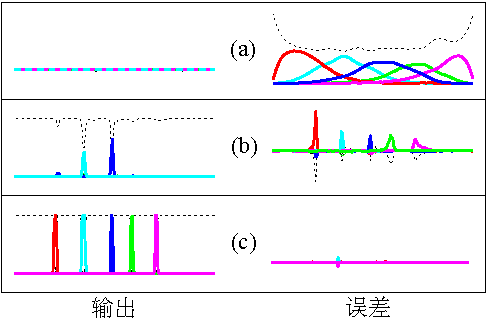
\includegraphics[width=\columnwidth]{fig/4}
	\caption{\textbf{训练过程中,CTC~误差信号的变化}.左边一列展示了同一个序列在训练不同阶段的输出激活值(虚线是空符号的单元);右边一列展示了相应的误差信号.横轴上方的误差会相应增加到输出激活值上,下方的会相应减少输出激活值.(a)开始时,网络具有较小的随机权重,误差只由目标序列确定.(b)网络开始作出预测,误差定位这些预测附近.(c)网络以高置信预测出正确的标注,误差几乎消失.}
\end{figure}
\section{实验}
\label{sec:experiments}
我们将~CTC~与~HMM~和~HMM-RNN~混合式系统的表现在对~TIMIT~语音语料进行语音标注这一真实的时序分类问题上进行比较.更确切地说,任务是用音素序列在~TIMIT~测试集中对语句(utterance)进行标注,且标签错误率尽可能低(见~\ref{sec:ler}~节中的定义).

公平起见,比较~CTC~和混合网络时使用了相同的~RNN~架构——双向长短期记忆模型(bidirectional Long Short-Term Memory, BLSTM; \citealp{graves2005bidirectional}).BLSTM综合了长短期记忆模型(Long Short-Term Memory, LSTM; \citealp{hochreiter1997long})能记忆长时信息和双向~RNN(bidirectional RNN, BRNN; \citealp{schuster1997bidirectional})能看到过去和未来上下文的优点.需要强调的是,可以使用其他任何合理的架构.我们选择~BLSTM~是因为我们在同样任务上使用标准~BRNN~和单向网络的结果相对较差.
\subsection{数据}
TIMIT~语料库中是录制的英语语音,提供要念的文稿给说话人.样本带有人工切分好的音标.词典(lexicon)中包含$61$个不同的音素(phoneme),被分为训练集和测试集,分别包含$4620$和$1680$个语句.从训练用语句中随机选出$5$\%($184$),在混合系统和~CTC~的实验中用作早终止(early stopping)所需的验证集.音频数据切为$10$ms长的帧,两帧之间重叠$5$ms,使用$26$个滤波器组信道(filter-bank channels)上的$12$个梅尔频率倒谱系数(Mel-Frequency Cepstrum Coefficients, MFCC).此外还使用了对数能量和各系数的一阶导数,这样对每帧得到一个$26$维的系数向量.我们在训练集上将系数逐一归一化,使总体分布遵循$0$均值$1$标准差.
\subsection{实验设置}
CTC~网络使用的是带有窥孔(peephole)和遗忘门(forget gate)的扩展~BLSTM~结构\citep{gers2003learning},每个前向和后向隐层中有$100$个记忆块,输入和输出单元采用$\tanh$激活函数,门采用的是值域为$[0,1]$的对数几率~sigmoid~函数.

隐层和自身及输出层间是全连接的,此外还有来自输入层的全连接.输入层大小为$26$,softmax~输出层大小为$62$($61$类音素加上空字符标签),共$114662$个权重.

训练以时间反向传播和在线梯度下降(online gradient descent)完成(权重在每个训练示例后更新),使用$10^{-4}$的学习率,动量设为$0.9$.在学习每个样本前,将网络的激活值重置为$0$.对前缀搜索解码(\ref{sec:classifier}~节),空符号的概率阈值设置为$99.99$\%.权重以$[-0.1,0.1]$上的均匀分布初始化.在训练期间,加入了标准差为$0.6$的高斯噪声以提高泛化.

基线~HMM~和混合式系统按\citep{graves2005framewise}的描述实现.简单来说,基线~HMM~采用了上下文无关模型和含三个状态、自左向右的上下文相关模型,模型利用~HTK~工具包\footnote{\url{http://htk.eng.cam.ac.uk/}}进行训练和测试.观测概率用高斯混合模型建模.高斯分布的个数和插入损失(insertion penalty)经过选择,以取得任务上的最优性能.系统中不包含语言学信息,也不包含部分音素序列(partial phone sequence),共计$90$多万个参数.

混合式系统中包含~HMM~和一个~BLSTM~网络,用基于~Viterbi~算法的强制对齐(forced alignment)进行训练\citep{robinson1994an}.对$61$个音素的单状态模型,其转移概率和先验概率的初始估计在训练集上用正确的转写结果得出.选择了可取得任务上最优性能的插入损失.

BLSTM~的架构和参数与~CTC~使用的基本相同,区别在于:(1)混合式系统中,网络的学习率为$10^{-5}$;(2)加入的噪声标注差为$0.5$;(3)输出层有$61$个单元而非$62$个(没有空符号).两个系统的噪声水平和学习率经参数空间中的粗搜索后分别加以设置.混合式系统中的网络共有$114461$个权重,HMM~额外还需要$183$个参数.在误差加权实验中,对误差信号进行缩放,使得长音素和短音素的权重相同\citep{robinson1991several}.
\subsection{实验结果}
表~\ref{fig:1}~中的结果表明,采用前缀搜索解码的~CTC~性能比采用相同~RNN~结构的基线~HMM~识别器和~HMM-RNN~混合式系统均更优.结果还表明,前缀搜索解码相较最优路径解码性能略有提升.

注意,混合式系统上的最优结果是采用加权误差信号得到的. CTC不需要这样的启发式规则,因为它的目标函数只依赖于标签\textbf{序列},而与其长度和切分无关.

输入中的噪声对~CTC~的泛化影响比混合式系统要大,而对~CTC~而言,最优的噪声水平要高一些.
\begin{table}
	\centering
	\caption{\textbf{TIMIT~上的标签错误率(LER)}. CTC~和混合式系统的结果是五次的均值$\pm$标准差.除误差加权~BLSTM/HMM~和~CTC(最优路径解码)外,差异均非常显著($p<0.01$).}
	\label{table:1}
	\begin{tabular}{ll}
		\hline
		系统            & LER \\ \hline
		上下文无关~HMM      &  $38.85$\%   \\
		上下文相关~HMM      &  $35.21$\%   \\
		BLSTM/HMM     &  $33.84\pm 0.06$\%   \\
		误差加权~BLSTM/HMM &  $31.57\pm 0.06$\%   \\
		CTC(最优路径解码)   &  $31.47\pm 0.21$\%   \\
		CTC(前缀搜索解码)   &  $30.51\pm 0.19$\%  \\ \hline
	\end{tabular}
\end{table}
\section{讨论和未来工作方向}
\label{sec:discussion}
CTC~和其他时序分类器之间的一个关键区别是~CTC~并不显式切分其输入序列.这有几点好处,包括不再需要定位固有不明确的标签边界(如语音识别和手写体识别中),此外,如果有帮助的话允许将标签预测分组在一起(比如某几个标签经常一起出现时).总之,如果只需要标签序列,为确定切分而进行建模便是一种浪费.

对于需要分割的任务(例如蛋白质二级结构预测),使用~CTC~似乎有问题.但是,从图~\ref{fig:1}~中可以看出,CTC~自然倾向于将每个标签预测与序列的相应部分对齐.因此它应该适用于关键字发现(keyword spotting)之类只需要近似切分的任务.

CTC~的另一个显著特征是它没有显式建模标签间的依赖关系.这不同于通常假定标签构成$k$阶马尔可夫链的图模型.不过,CTC~\textbf{隐含地}建模了标签间的依赖关系.例如,它会以双峰(double spike)的形式预测共现的标签(见图~\ref{fig:1}).

处理结构化数据的一种非常普遍的方式是时序分类器的层次结构,其中一个层次的标签(例如字母)成为下一个标签(例如字)的输入.采用分层~CTC~的初步实验令人鼓舞,我们打算进一步推进这一方向.

应用最大似然训练时,想要较好地泛化总是很困难,但~CTC~似乎尤然.未来我们将继续探索减少过拟合的方法,如权重衰减(weight decay)、提升(boosting)和边缘最大化(margin maximisation).
\section{结论}
\label{sec:conclusion}
我们介绍了一种用~RNN~进行时序分类的通用新方法.这一方法与神经网络分类器的已有框架自然吻合,且由同一套概率原理导出.它避免了预先切分数据的需要,可以直接训练网络进行序列分类.此外,不利用与领域相关的知识,它在一个真实时序分类问题上的表现就超越了~HMM~和~HMM-RNN~混合式系统.

\section*{致谢}
感谢~Marcus Hutter~在数学方面的有益讨论.本研究得到了~SNF~基金~200021-111968/1及200020-107534/1~的支持.

% TODO: 加引用
\bibliography{cites}
\bibliographystyle{icml2017}

\end{document} 
